\documentclass[
12pt,
a4paper,
pdftex,
czech,
titlepage
]{report}

\usepackage[czech]{babel}
\usepackage[utf8]{inputenc}
\usepackage{lmodern}
\usepackage{textcomp}
\usepackage[T1]{fontenc}
\usepackage{amsfonts}
\usepackage{titlesec}
\usepackage{graphicx}
\usepackage{framed}
\usepackage{amsmath}

\titleformat{\chapter}
  {\normalfont\LARGE\bfseries}{\thechapter}{1em}{}
\titlespacing*{\chapter}{0pt}{0ex plus 1ex minus .2ex}{2.0ex plus .2ex}
\setlength\parindent{0pt}

\begin{document}

\begin{titlepage}
	\vspace*{-2cm}
	{\centering
\includegraphics[scale=1.0]{logo.pdf}\par}
	\centering
	\vspace*{2cm}
	{\Large Semestrální práce z KIV/PC\par}
	\vspace{1.5cm}
	{\Huge\bfseries Vyhledávání cest v grafu technikou DFS\par}
	\vspace{2cm}

	{\Large Petr Hlaváč\par}
	{\Large A15B0037P\par}
	{\Large petrh@students.zcu.cz\par}

	\vfill

	{\Large 6.\,12.\,2017}
\end{titlepage}

\tableofcontents
\thispagestyle{empty}
\clearpage

\chapter{Zadání}
Naprogramujte v ANSI C přenositelnou \textbf{konzolovou aplikaci}, která bude \textbf{procházet graf technikou DFS} (Depth--First--Search). Vstupem aplikace bude soubor s popisem grafu. Výstupem je pak odpovídající výčet všech cest mezi požadovanými uzly.\\

Program se bude spouštět příkazem \textbf{dfs.exe} <soubor-grafu> <id1> <id2> <maxD>
\begin{itemize}
\item Symbol <soubor-grafu> zastupuje parametr - název vstupního souboru se strukturou grafu.
\item Následují identifikátory (dále jen id) dvou uzlů v grafu <id1> a <id2>, mezi kterými bude spouštěn proces hledání cest.
\item <maxD> je parametr popisující maximální délku cest, které mají být nalezeny.
\end{itemize}

Vámi vyvinutý program tedy bude vykonávat následující činnosti.
\begin{enumerate}
\item Při spuštění bez potřebných parametrů vypíše nápovědu pro jeho správné spuštění a ukončí se.
\item Při spouštění s parametry načte zadaný vstupní soubor do vhodné struktury reprezentující graf a mezi zadanými uzly najde všechny cesty, jejichž délka nepřekročí konstantu nastavenou vstupním parametrem.
\end{enumerate}

Váš program může být během testování spuštěn například takto:\\

\framebox[1.1\width]{dfs.exe graph.csv 1 2 4}\\

Při tomto spuštění program vyhledá všechny cesty délky 1 až 4 mezi uzly 1 a 2.\\

Hotovou práci odevzdejte v jediném archivu typu ZIP prostřednictvím automatického odevzdávacího a validačního systému. Postupujte podle instrukcí uvedených na webu předmětu. Archiv nechť obsahuje všechny zdrojové soubory potřebné k přeložení programu, \textbf{makefile} pro Windows i Linux a dokumentaci ve formátu PDF vytvořenou v typografickém systému \TeX, resp. \LaTeX.

\section{Popis činnosti programu}
Program načte vstup ve formátu CSV, který vhodným způsobem uloží do paměti pro pozdější prohledávání. Následně spustí algoritmus, jehož výstupem bude seznam všech cest mezi dvěma uzly, které bude vypisovat na standardní výstup ve formátu popsaném dále.

\subsection{Specifikace výstupu programu}
Program bude na standardní výstup vypisovat jednotlivé cesty. Vždy na jeden řádek právě jednu cestu. Cesty budou popsány posloupností id jednotlivých uzlů oddělených pomlčkou (tj. znakem minus,  \uv{\textbf{-}}). Následovat bude středník a popisky jednotlivých hran v grafu oddělené čárkou. Za posledním středníkem bude uvedena hodnota sekundární metriky - relevance cesty, podle které budou cesty seřazeny (viz Řazení výstupu).\\

Například tedy pro hledání cest mezi uzly A a B:\\

\textbf{A-B};$h_{1}$;$m_{1}$\\
\textbf{A-F-B};$h_{2}$,$h_{3}$;$m_{2,3}$\\
\textbf{A-W-B};$h_{4}$,$h_{5}$;$m_{4,5}$\\
\textbf{A-F-O-B};$h_{2}$,$h_{6}$,$h_{7}$;$m_{2,6,7}$\\


Kde A, B, F, W, F, ... jsou popisky uzlů grafu, $h_{n}$ jsou ohodnocení hran a $m_{c1,c2...cn}$ je hodnota metriky relevance nalezené cesty.

\subsection{Řazení výstupu}
Cesty budou na standardním výstupu seřazeny podle jejich délky. Pokud bude nalezeno více cest stejné délky, budou seřazeny podle jejich relevance následujícím způsobem. Popisky grafu nesou informaci o kalendářním datu ve formátu YYYY--MM--DD. Každá cesta bude tedy ohodnocena celým číslem, které bude odpovídat rozdílu v počtu dní mezi nejstarším a nejnovějším datem, následně budou podle tohoto čísla cesty se shodnou délkou seřazeny vzestupně.\\


\newpage
Pokud tedy nalezete cestu, kterou budou tvořit tyto 4 hrany s hodnotami:\\

2000--01--15,\\
2000--01--04,\\
2000--01--19,\\
2000--01--24,\\

vypočte se hodnota metriky jako počet dnů mezi daty 2000--01--04 a 2000--01--24, což je 20.

\section{Podrobné zadání}
Originální nezkrácené zadání je možné nalézt na adrese:\\

http://www.kiv.zcu.cz/studies/predmety/pc/doc/work/sw2017-02.pdf

\setcounter{page}{1}

\chapter{Analýza úlohy}
Úloha se skládá z následujících kroků:
\begin{enumerate}
	\item Načtení vstupních dat.
	\item Vybrání vhodné datové struktury.
	\item Modifikace algoritmu DFS pro hledání všech cest mezi dvěma body.
	\item Vypisování výsledných cest.
\end{enumerate}

\section{Načtení vstupních dat}
CSV nebo-li Comma-separeted-values je jednoduchý souborový formát určený pro výměnu tabulkových dat.\\

Ukázka vstupního souboru ve formátu CSV
\begin{framed}
	1;2;2007--02--16\\
	1;2;2008--02--15\\
	1;3;2007--10--26\\
	1;4;2007--10--30\\
	3;2;2007--10--11\\
	3;6;2007--06--14\\
	3;7;2007--08--14\\
	3;9;2008--03--05\\
	4;2;2007--10--05\\
	5;1;2007--02--04
\end{framed}

Data jsou formátovány ve stylu idUzlu1; idUzlu2; hodnotaHrany\\

Jedna řádka vstupního souboru představuje jednu hranu. Bude tedy vhodné načítat a zpracovávat data po řádcích. Formát CSV nám práci s daty velmi ulehčí, neboť nebude příliš náročné data v řádce rozdělit za pomoci znaku~\uv{\textbf{;}}.

\section{Vybrání vhodné datové struktury}
Pro reprezentaci grafu se využívají následující struktury:
\begin{enumerate}
	\item Matice sousednosti
	\item Spojový seznam
\end{enumerate}

\subsection{Matice sousednosti}
Matice sousednosti má velikost $V \times V$, kde $V$ je počet uzlů. Vzhledem k faktu, že máme ohodnocené hrany grafu, vložíme na pozice v matici, kde se nachází hrana její hodnotu a na pozice, kde hrana není, vložíme nějakou speciální hodnotu, v našem případě (NULL). Hrany v grafu jsou zadány jako neorientované, tudíž matice bude symetrická, viz vzorová matice sestavená pro výše zmíněná vstupní data. Hodnota NULL je v matici nahrazena znakem \uv{--}\\

$\begin{matrix}
 0 & 1 & 2 & 3 & 4 & 5 & 6 & 7 & 8 & 9 \\
 1 & - & h1,h2 & h3 & h4 & h10 & - & - & - & - \\
 2 & h1,h2 & - & h5 & h9 & - & - & - & - & - \\
 3 & h3 & h5  & - & - & - & h6 & h7 & - & h8 \\
 4 & h4 & h9 & - & - & - & - & - & - & - \\
 5 & h10 & - & - & - & - & - & - & - & - \\
 6 & - & - & h6 & - & - & - & - & - & - \\
 7 & - & - & h7 & - & - & - & - & - & - \\
 8 & - & - & - & - & - & - & - & - & - \\
 9 & - & - & h8 & - & - & - & - & - & - \\
\end{matrix}$\\

Neboť je matice pro orientované hrany symetrická, lze ji z paměťových důvodů polovinu zanedbat.
Uložená matice by tedy vypadala takto.\\

$\begin{matrix}
0 & 1 & 2 & 3 & 4 & 5 & 6 & 7 & 8 & 9 \\
1 & -  \\
2 & h1,h2 & -  \\
3 & h3 & h5  & -  \\
4 & h4 & h9 & - & -  \\
5 & h10 & - & - & - & -  \\
6 & - & - & h6 & - & - & - \\
7 & - & - & h7 & - & - & - & - \\
8 & - & - & - & - & - & - & - & -  \\
9 & - & - & h8 & - & - & - & - & - & - \\
\end{matrix}$\\

Pokud se na tuto matici podíváme pozorně, zjistíme že jde v podstatě o reprezentaci Spojovým seznamem. Jedinou výhodou je přístup na dané hrany ve složitosti $O(1)$, neboť matice je reprezentována polem. Tato výhoda má ale ovšem i negativa. Spočívají v tom, že je třeba uložit pole, které je stejně veliké jako id největšího vrcholu v našem grafu. V případě, který nastal i zde, je tedy možné, že budeme mít v maticí řádky, které jsou uloženy zcela zbytečně například řádek číslo 8.\\

Další nevýhodou, které si můžeme všimnout, je násobnost hran. Abychom v matici uchovali více hran mezi dvěma vrcholy, musí být hrany v matici reprezentovány spojovým seznamem nebo polem. V případě volby pole by každé přidání nové hrany znamenalo zvětší pole o jedna a přepsání všech hodnot do nového pole, což je v při načítání velkého grafu velmi neefektivní. Vhodnější je tedy spojový seznam.\\

Výsledkem této reprezentace je tedy matice spojových seznamů. Velkou výhodou je přístup k hranám vrcholů v $O(1)$. Nevýhodou může být v některých případech grafů zbytečně velká paměťová složitost a také složitost implementace.


\subsection{Seznam sousednosti}
Struktura seznamu sousednosti znamená, že máme pro každý vrchol vytvořen spojový seznam hran, které z něho vycházejí a v kterých je uloženo id souseda a ohodnocení hrany. Spojový seznam pro výše zmíněna data by vypadal takto.\\

\begin{figure}[!h]
	\centering
	 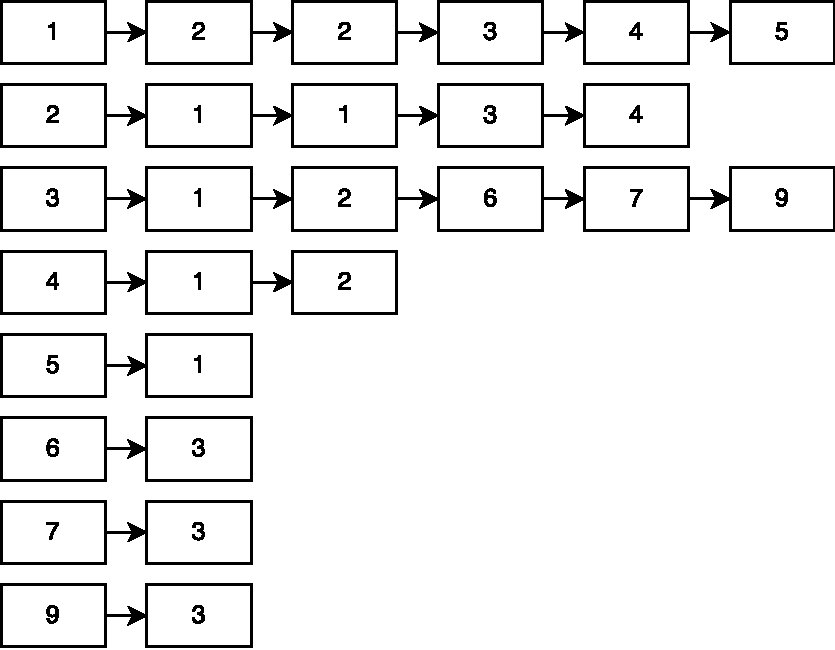
\includegraphics[scale=0.5]{spojak.pdf}
	\caption{Reprezentace grafu spojovým seznamem}
\end{figure}

Neorientované hrany jsou vyřešené přidáním stejné hrany k oběma vrcholům. Násobné hrany v této implementaci nedělají žádný problém.\\

Vrcholy grafu je možné mít uložené v poli nebo spojovém seznamu. Výhoda pole je přístup k hraném v $O(1)$. Nevýhodou je paměťová náročnost v případě nevyužití všech indexů pole. Spojový seznam má přístup k vrcholům v $O(n)$, což může program značně zpomalovat v případě velkého počtu vrcholů v grafu. Vhodná volba tedy záleží hlavně na znalosti vstupních dat.

\section{Modifikace algoritmu DFS}
Vyjdeme ze základního algoritmu DFS neboť nám byl pevně stanoven zadáním úlohy.

\subsection{Ukončovací podmínky}
 Ze zadání víme, že naše prohledávání bude omezeno hloubkou. Dále bylo také řečeno, že se jedná o cestu. Cesta v grafu je definována jako posloupnost vrcholů ve které není žádný vrchol obsažen dvakrát. Známe tedy dvě hlavní podmínky pro ukončení prohledávání do hloubky. První je maximální hloubka, kterou dostaneme zadanou při spuštění programu a druhá je v případě, že aktuální hledaná cesta již obsahuje daný vrchol.
 
 \subsection{Ukládání cest}
  Nyní již máme vhodný způsob jak v daném grafu cesty hledat. Bylo by ale také vhodné si je někam ukládat. Budeme si proto při každém nalezení vrcholu ukládat předchůdce, nebo-li vrchol ze kterého jsme se do nově nalezeného vrcholu dostali. Vznikne nám tedy u každého vrcholu seznam předchůdců. Pokud půjdeme po jednotlivých předchůdcích, dostaneme cestu z daného vrcholu do vrcholu, ze kterého jsme prohledávání začali. Vrchol bude obsahovat tolik předchůdců, kolik existuje cest z výchozího vrcholu do námi zkoumaného vrcholu.\\
  
  Seznam předchůdců pro jednotlivé vrcholy by pro vzorová vstupní data a vzorové spuštění programu vypadal takto:\\
  
  1()\\
  2(1,1,3,4)\\
  3(2,2,1,2)\\
  4(2,2,2,1)\\
  5(1)\\
  6(3,3,3,3)\\
  7(3,3,3,3)\\
  9(3,3,3,3)\\
  
  Hodnota před závorkou značí id vrcholu, hodnoty v závorce pak id předchůdců.
  Při přidávání předchůdců bude také vhodné přidávat ohodnocení jejich hran, aby bylo možné zpětně sestavit i ohodnocení dané cesty.
  
  \section{Vypisování výsledných cest}
  Vzhledem k metodě ukládání cest nemáme cesty seřazené ani podle ohodnocení, ani podle délky. Nejvhodnější tedy bude u každé cesty vypočítat její ohodnocení a délku, a poté je setřídit.\\
  
  Setřízení je možné provést více způsoby například:
  
  \begin{enumerate}
  	\item Polem - kde uložíme id cesty,ohodnocení a délku, následně pole uspořádáme a budeme cesty vypisovat podle jednotlivých indexů.
  	\item Spojovým seznamem - kde nově přidanou cestu zařadíme na pozici určenou jejím ohodnocením.
  \end{enumerate}

	Spojový seznam se zde zdá jako vhodnější varianta, neboť výsledkem bude uspořádaný seznam cest, které už bude stačit pouze vypsat ve formátu uvedeném v zadání.

\chapter{Implementace}
Dle zadání byla sestavena přenositelná konzolová aplikace naprogramována v jazyce ANSI C. Program je rozdělen do 9 modulů. Každá část kromě (\textbf{main}) se skládá z hlavičkového souboru s příponou .h a zdrojového textu s výkoným kódem s příponou .c.

\begin{enumerate}
	\item main
	\item dataloader
	\item date
	\item graph
	\item neighbours
	\item paths
	\item predecessors
	\item search
	\item stack
\end{enumerate}

\section{main}
Modul main se stará o kontrolu argumentů převzatých z příkazové řádky. Kontroluje jejich počet, správný typ a předává je modulu dataloader a modulu search. Při špatném počtu parametrů vypíše návod jak správně aplikaci spustit. V případě nevalidního parametru vypíše, který to byl.

\section{dataloader}
Modul dataloader se stará o načítání dat ze souboru a vytváří z nich datovou strukturu grafu. Data jsou načítány po řádcích funkcí \textbf{fgets()}. Jako maximální počet znaků načtených z řádky je zvolena hodnota 36. K tomu číslu jsme dospěli započítáním počtu znaků dvou integerů, dvou středníků a data ve formátu YYYY-MM-DD. Poté je pomocí funkce \textbf{strtok()} rozdělen na data idUzlu1, idUzlu2 a hodnotuHrany. Tyto informace jsou uložené do datové struktury v modulu graph.

\section{date}
Modul date je pouze podmnožinou struktury tm z modulu <time.h>. Obsahuje celkem 3 hlavní funkce. První je vytvoření struktury date z textu ve formátu YYYY-MM-DD, druhá je porovnání dvou dat. Poslední funkce slouží k získání rozdílu dvou dat ve dnech. Tato funkce je realizována pomocí modulu <time.h> a jeho metody \textbf{difftime()}.

\section{graph}
Modul graph má na starosti datovou strukturu grafu. Graf je implementován pomocí spojového seznamu vrcholů. Každý vrchol obsahuje svoje id a seznam sousednosti z modulu Neighbours.

\section{neighbours}
Modul neighbours je spojový seznam hran v grafu. Hrana je reprezentována strukturou edge. Každá struktura edge obsahuje ohodnocení a ukazatel na vrchol grafu do kterého směřuje.

\section{paths}
Modul paths se skládá ze dvou částí. První část je struktura path, což je spojový seznam, který obsahuje vrcholy a hrany z kterých se cesta skládá. Tato struktura také obsahuje délku cestu a udržuje informaci o nejnovějším a nejstarším datu v cestě pro výpočet výsledného ohodnocení cesty. Informace o datu a dálce je aktualizována s každým přidáním dalšího prvku do listu. Druhou částí je setřízený spojový seznam všech cest. Jde o spojový seznam, do kterého vkládáme výše zmíněné cesty. Cesta je vložena na své místo v seznamu dle její délky a ohodnocení.

\section{predecessors}
Modul predecessors se skládá také z dvou částí. První je seznam předchůdců. Je složen z jednotlivých odkazů na id vrcholu, ze kterého byl aktuální vrchol přidán, ohodnocení hrany, která bylo využita a odkazu na dalšího předchůdce. Tento seznam je unikátní pro každý vrchol v grafu a proto nese vlastní identifikátor podle id vrcholu. Všechny seznamy předchůdců jsou následně uloženy do výsledného seznamu, který slouží k zjištění stavu prohledávání.

\section{search}
Modul search obsahuje metodu prohledávání do hloubky. Tento modul byl vytvořen s tím, že v budoucnu by mohl obsahovat další metody vyhledávání cest v grafu například modifikovaným Dijstrovým nebo BFS algoritmem.

\section{stack}
Modul stack obsahuje datovou strukturu zásobník. Nový prvek do zásobníku se přidává na začátek a v případě volání funkce \textbf{pop} je ze zásobníku první prvek odstraněn a vrácen návratovou hodnotou funkce. Zásobník je implementován pro strukturu stack node, která obsahuje vrchol na který se přechází, ohodnocení využité hrany, úroveň hloubky prohledávání a ukládá předchozí vrchol jako předchůdce.

\chapter{Uživatelská příručka}
\section{Přeložení programu}
Pro překlad je zapotřebí překladač gcc. K programu je přiložen soubor Makefile a lze ho tedy snadno přeložit tím, že se v příkazovém řádku přepneme do složky se zdrojovými soubory a zavoláme příkaz na sestavení. Na Linuxu je to příkaz make na Windowsu mingw32-make.

\section{Spuštění programu}
Program lze spustit z příkazové řádky příkazem ./dfs <parametry> na systému Linux a dfs <parametry> na systému Windows.\\

Parametry pro spuštění jsou <soubor-grafu> <id1> <id2> <maxD>
\begin{itemize}
	\item Symbol <soubor-grafu> zastupuje parametr - název vstupního souboru se strukturou grafu.
	\item Následují identifikátory (dále jen id) dvou uzlů v grafu <id1> a <id2>, mezi kterými bude spouštěn proces hledání cest.
	\item <maxD> je parametr popisující maximální délku cest, které mají být nalezeny.
\end{itemize}

Při spuštění s jiným počtem parametrů program vypíše nápovědu jak ho správně spustit. V případě nevalidní parametru je vypsáno, který to byl. 

\chapter{Závěr}
Program byl napsán tak, aby byl snadno rozšířitelný. Moduly jsou připraveny k implementaci více druhů prohledávání grafu. Z výsledku by mohlo vzniknout hezké poměření algoritmů při řešení tohoto NP-úplného problému.\\
V případě prohledávání pouze grafů, kde víme že id vrcholu je kladné číslo v rozsahu od $<0,2147483647>$ by mohlo být programování značně urychleno reprezentací Matice sousednosti a ukládáním jak vrcholu grafu, tak předchůdců v grafu do pole, místo do spojového seznamu. Bohužel tato informace nebyla nikde dána. Bylo tedy zvoleno více univerzální řešení, které je pomalejší.\\
Práce byla vytvářena déle než na portále naivně uvedených 40 hodin. Zejména velkou část času spotřebovala dokumentace v \LaTeX, který s předmětem jako takovým nemá nic společného. Bylo zajímavé si vyzkoušet práci s nízkoúrovňovým programovým jazykem, avšak po několika hodinách práce bylo jasné, proč tento jazyk poslední roky ztrácí na oblibě.\\
Validace pomocí validátoru se zdá býti poněkud neštastná. V případě ,že i maličkost není v zadání řádně specifikována. Může to véct k tomu, že student stráví nad validací 2 dny, jako se stalo v tomto případě. Validátor přitom v hodnocení práce nehraje žádnou roli, neboť je hodnocena ručně.

\end{document}